
\documentclass[twocolumn]{book}

\usepackage{graphicx}
\usepackage{hyperref}

\title{Maps and Notes to Supplement Churchill's {\it A History of the
English-Speaking Peoples\/}}

\author{Thomas E.~Vaughan}

\begin{document}

\frontmatter

\maketitle

\chapter{Preface}

Winston Churchill's {\it A History of the English-Speaking Peoples\/} is an
excellent history, but, at least in its abridgment for the American audience,
the book lacks maps. A reader like me, lacking proper knowledge of geography
and of the evolution of place names over time, will have some difficulty in
visualizing the location of one or another event. The present work is an effort
to provide a visual reference for Churchill's book.

Unless indicated otherwise by the text in the present work, every page number
refers to Churchill's book, and every quotation comes from Churchill's book.
The source for each map is given in its caption.

\mainmatter%

\chapter{Britannia}

On Page~1 is a reference to Gaul, which Julius Caesar had conquered by 55~BC\@.
Figure~\ref{fig:gaul-bc} depicts the Roman view of Gaul at the time. Gaul
covered the territory now covered by France, Luxembourg, Belgium, part of the
Netherlands, and part of Germany.  After conquering Gaul, Caesar turned his
attention to Brittania, whose people were of the same Celtic culture as those
in Gaul. ``The Islanders had helped the local tribes in the late campaigns
along the northern coast of Gaul\ldots.  British volunteers had shared the
defeat of the Veneti on the coasts of Brittany in the previous year.'' The
location of the Veneti is indicated in Figure~\ref{fig:gaul-bc}, and Brittany
is located in Figure~\ref{fig:brittany}.

\begin{figure}
   \begin{center}
      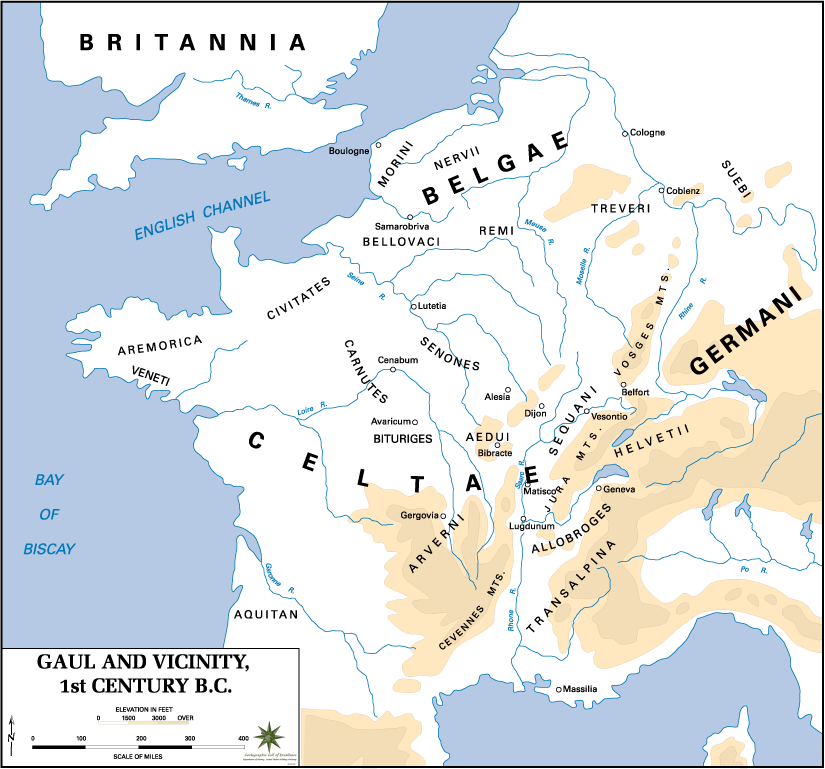
\includegraphics[width=0.9\columnwidth]{images/Gaul-1st-century-BC}
      \caption{%
         Gaul as viewed by the Romans in the First Century BC\@.
         \url{http://en.wikipedia.org/wiki/Gauls}%
      }\label{fig:gaul-bc}
   \end{center}
\end{figure}

\begin{figure}
   \begin{center}
      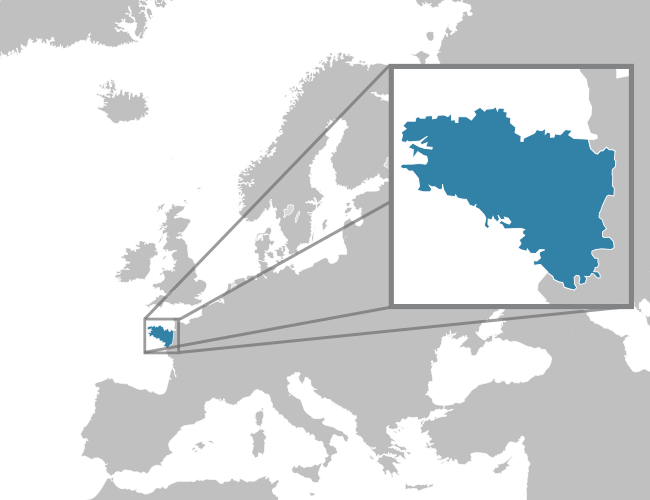
\includegraphics[width=0.9\columnwidth]{Bretagne}
      \caption{%
         Brittany's location in northwest France\@.
         \url{http://en.wikipedia/org/wiki/Brittany}
      }\label{fig:brittany}
   \end{center}
\end{figure}

\begin{figure}
   \begin{center}
      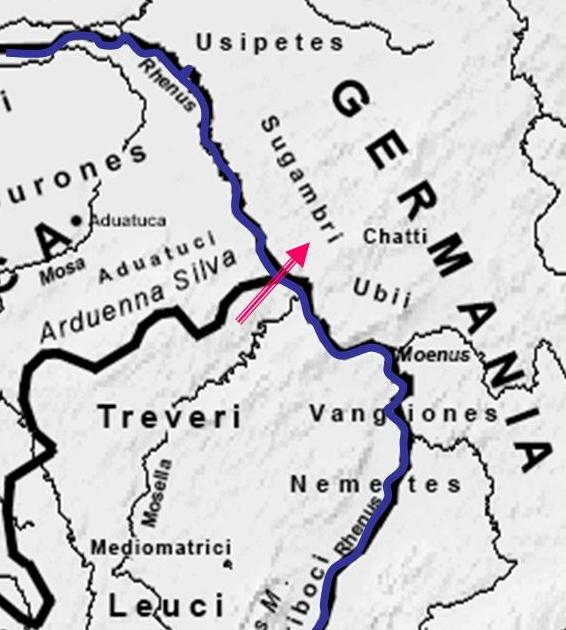
\includegraphics[width=0.9\columnwidth]{images/Rhine-Crossing}
      \caption{%
         Location of Caesar's Rhine crossing\@.
         \url{http://en.wikipedia/org/wiki/Caesar's_Rhine_bridges}
      }\label{fig:Rhine-Crossing}
   \end{center}
\end{figure}

\begin{figure}
   \begin{center}
      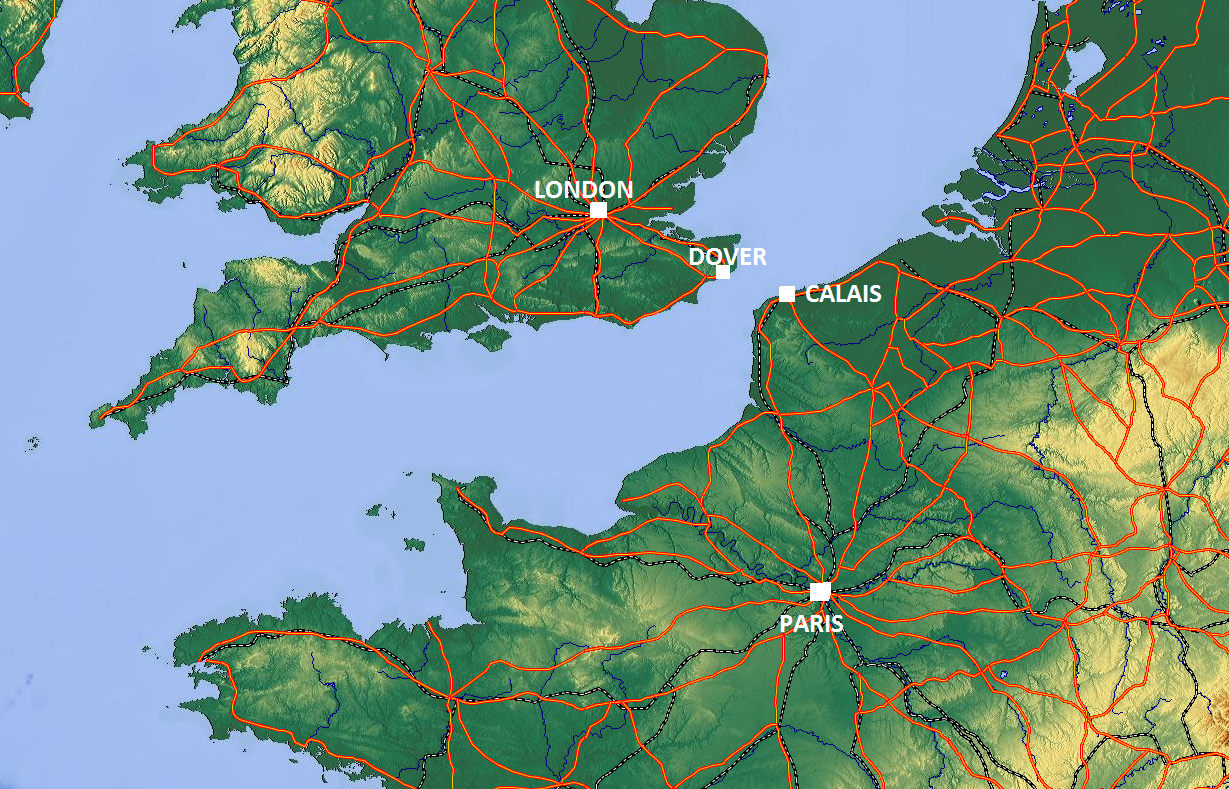
\includegraphics[width=0.9\columnwidth]{images/LondonCalaisParis}
      \caption{%
         Location of Calais\@.
         \url{http://en.wikipedia/org/wiki/Calais}
      }\label{fig:LondonCalaisParis}
   \end{center}
\end{figure}

\begin{figure}
   \begin{center}
      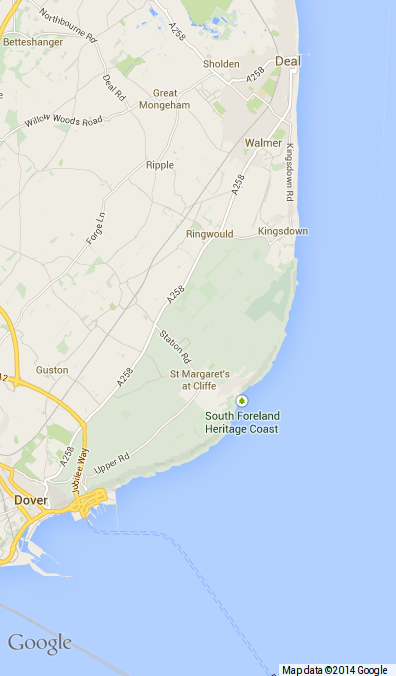
\includegraphics[width=0.9\columnwidth]{images/DoverDealWalmer}
      \caption{%
         Location of Deal and Walmer\@.
         \url{https://www.google.com/maps/@51.179681,1.3039197,12z}
      }\label{fig:DoverDealWalmer}
   \end{center}
\end{figure}

On Page~2 is a reference to Caesar's timber bridge across the Rhine above
Coblenz, whose location can be found in Figure~\ref{fig:gaul-bc}. A magnified
view is provided in Figure~\ref{fig:Rhine-Crossing}. The bridge is regarded as
a marvel of military engineering. After the bridge was destroyed, Caesar
marched his troops westward to the shore somewhere between Boulogne and Calais.
The location of Boulogne can be found in Figure~\ref{fig:gaul-bc}. The location of
Calais can be found in Figure~\ref{fig:LondonCalaisParis}.

``Late in August 55 B.C.~Caesar sailed with eighty transports and two legions
at midnight, and with the morning light saw the white cliffs of Dover crowned
with armed men.'' The location of Dover, just opposite the English Channel from
Calais, is depicted in Figure~\ref{fig:LondonCalaisParis}. ``He judged the
place `quite unsuitable for landing', since it was possible to throw missiles
from the cliffs on to the shore. He therefore anchored till the turn of the
tide, sailed seven miles farther, and descended upon Albion on the low,
shelving beach between Deal and Walmer.'' The relationships among Dover, Deal,
and Walmer can be seen in Figure~\ref{fig:DoverDealWalmer}.

\backmatter%

\end{document}

